\section{Highlights}

\subsection{``Real'' EARS}

A significant amount of effort was invested into making \textsf{EARS-CTRL} as close as
possible to the real EARS templates used at Rolls-Royce. Given the fact that
EARS was not originally built to describe requirements at a level where they can
automatically be transposed into a real system, a large investment was made into
having a translation from EARS into the formalism used by a controller
synthesizer (the Linear Temporal Logic -- LTL -- formalism) that would overcome 
as much as possible the barriers between the structured but non-formal nature of
EARS, and the strictly formal nature of LTL.

\begin{figure}[t]
   \begin{center}
     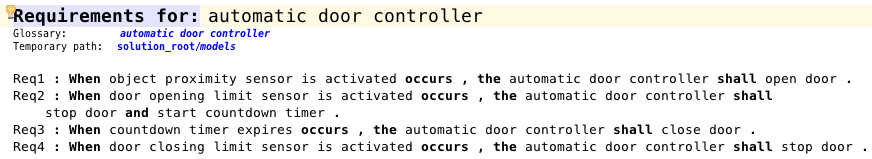
\includegraphics[width=1\textwidth]{images/EARS-Reqs.png}
     \caption{Requirements for a sliding door controller written using the 
     \textsf{EARS-Ctrl} editor}
     \label{fig:ears_reqs}
   \end{center}
 \end{figure}
 
Figure~\ref{fig:ears_reqs} ilustrates a set of \textsf{EARS-Ctrl} requirements
for the software controller for a sliding door. By remaining as close as
possible to the original EARS syntax our editor allows building requirements in
correct English that can easily read and undertood by humans. 

One of the main goals of our approach is to remain as faithful as possible to
the requirements-capturing method proposed by Mavin~\cite{}, thus retaining its advantages of \ldots, as
described in~\cite{}. In such as manner our tool benefits from all the research
and advantages of EARS described in the literature~\cite{}. In order to be able
to ``write'' EARS-like requirements, a first analysis of the problem needs to be
done in the shape of the creation of a of glossary for the problem at hand. Such
a glossary is specific to the domain of controllers and identifies the
components of the system to be controlled, which have sensors and actuators the
controller logic will use respectively as inputs and outputs.

In order to reach a functioning controller we then allow interacting with the
automatically generated synthesizer using Simulink. When necessary the engineer
can edit the EARS requirements, where necessary, to be able to generate
controllers exhibiting the expected behavior. This may come at the cost of
sacrificing some of the readabilty of the original EARS
requirements.\levi{blahblah}

\subsection{A Push-Button Approach}

Controllers can be fully automatically synthesized from EARS requirements into
controllers, at the push of a button. \ldots

\subsection{Verification}

Our \textsf{EARS-CTRL} tool provides a set of mechanisms for verification, in
particular \emph{Well-Formedness by Construction} when the specification is
being built and \emph{simulation} of the synthesized controllers by exercising the
controller manually using \textsf{simulink} as a back-end. We can also generate
test cases for controllers that can either be used to debug the controller by
analysing traces of execution of the controller or to be used as test-cases for
alternative implementations of the controllers which are not automatically
synthesized.

\subsubsection{Well-Formedness by Construction}

Well-Formedness by construction is enforced at two levels in \textsf{EARS-CTRL}:
on the one hand only valid EARS requirement templates can be used. When the
requirements engineer selects an EARS template, the corresponding sentence is
shown to her as a structure with placeholders. These structures provide a
first level of well-formedness, as only correct sentences can be written. The
second level of well-formedness is guaranteed by the fact that only valid
sensors or actuators can be chosen in those sentences' placeholders. This is
illustrated in figure~\ref{}.

Well-formedness allows writing syntactically correct \textsf{EARS-CTRL}
specifications. The semantics of such specifications is then given by the
\textsf{autoConf4} synthesizer in the form of a synchronous dataflow diagram,
which \textsf{EARS-CTRL} can display when synthesis is possible. In the cases
where synthesis is not possible the error code from the\textsf{autoConf4} tool
is lifted such that the requirements that prevent the controller from being
generated are pointed out. \levi{this is not done yet}

\subsubsection{Simulation}

Once a controller can be synthesized from a set of EARS requirements, it becomes
important to understand whether that controller behaves as expected. In order to
do so we have built a translator from synchronous dataflow diagrams into
\textsf{Simulink}, which then allows us to exercise the behavior of the
controller.

\subsubsection{Generation of Test Cases}

\textsf{EARS-CTRL} allows generating test cases directly from the EARS
requirements. Test cases are generated through the panel displayed in
figure~\ref{}. A test case consists of a sequence of $\langle
  input, output \rangle$ pairs, where each input is a vector of sensor states
  and each output a vector of actuator states. Note that individual sensors and
  actuators assume two states: ``0'': off; ``1'': on.

In the test generation panel the engineer can parameterize test generation by
providing the following values:
\begin{itemize}
  \item \emph{Test Sequence Length:} defines the maximum length of the $\langle
  input, output \rangle$ pair sequences to be generated.
  \item \emph{Allow parallel inputs:} enables or disables the possibility of
  having more than one sensor being active for inputs in the test case.
  \item \emph{Allow repeated inputs:} enables or disables having repeated inputs
  in the same test sequence. When enabled this parameter makes it such that
  an input vector cannot occur more than once in a test sequence (thus limiting
  the length of test sequences to the number of possible input vectors).
\end{itemize} 


\subsection{Code Generation}

Generation of C code can be achieved by running Simulink's code generator on the
Simulink model that is generated from the requirements EARS expressed in 
\textsf{EARS-CTRL}.
